\pagebreak
\subsection{Electrical Design}
\colorbox{yellow}{\parbox{\textwidth}{The electrical design provides the hardware required for the implementation of the software, the sensors for the control system and furthermore a communication interface to the BEXUS system. A global diagram with the electrical interfaces between the IRISC experiment and BEXUS balloon are shown in figure \ref{fig:elec-ACD}.}} %The main interfaces are the E-Link and the power. But also, the camera's/ telescope should be able to watch the sky from the gondola.}}
\vspace{-.5cm}
\begin{figure}[H]
	\centering
	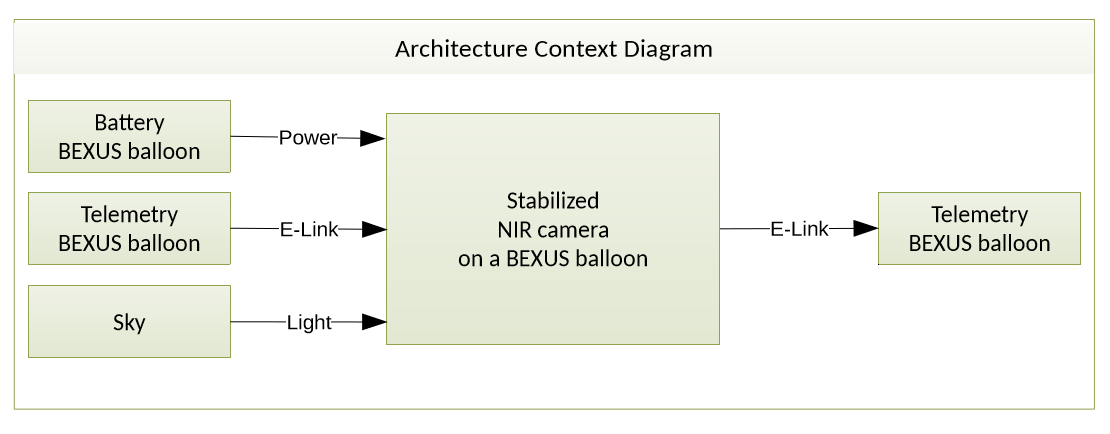
\includegraphics[width=.6\textwidth]{4-experiment-design/img/electrical/ArchitectureContext.png}
	\caption{Electrical architecture context diagram.}
	\label{fig:elec-ACD}
\end{figure}


\subsubsection{Block Diagram}
\label{sec:4.5.1}
\colorbox{yellow}{\parbox{\textwidth}{The architecture interconnect diagram of the electrical design is shown in figure \ref{fig:elec-AID}. The main controller is the Raspberry Pi. There is external storage for the obtained images. To stabilize the pictures the gyroscopes (relative) and encoders (absolute) are used. This will give enough information to stabilize the camera during one picture (accuracy $<$ 0.5 arcseconds required to achieve requirement P.8). Because the gondola also moves, a star tracker and GPS are used to measure this. Potentionally, an accelerometer and a compass will be used for additional complementary data. These only have to be accurate enough to have the target in the field of view of the camera ($<$ 0.5 degrees for the star tracker (P.9), $<$ 5 meters for the GPS (P.10)).}}
\vspace{-.5cm}
\begin{figure}[H]
	\centering
	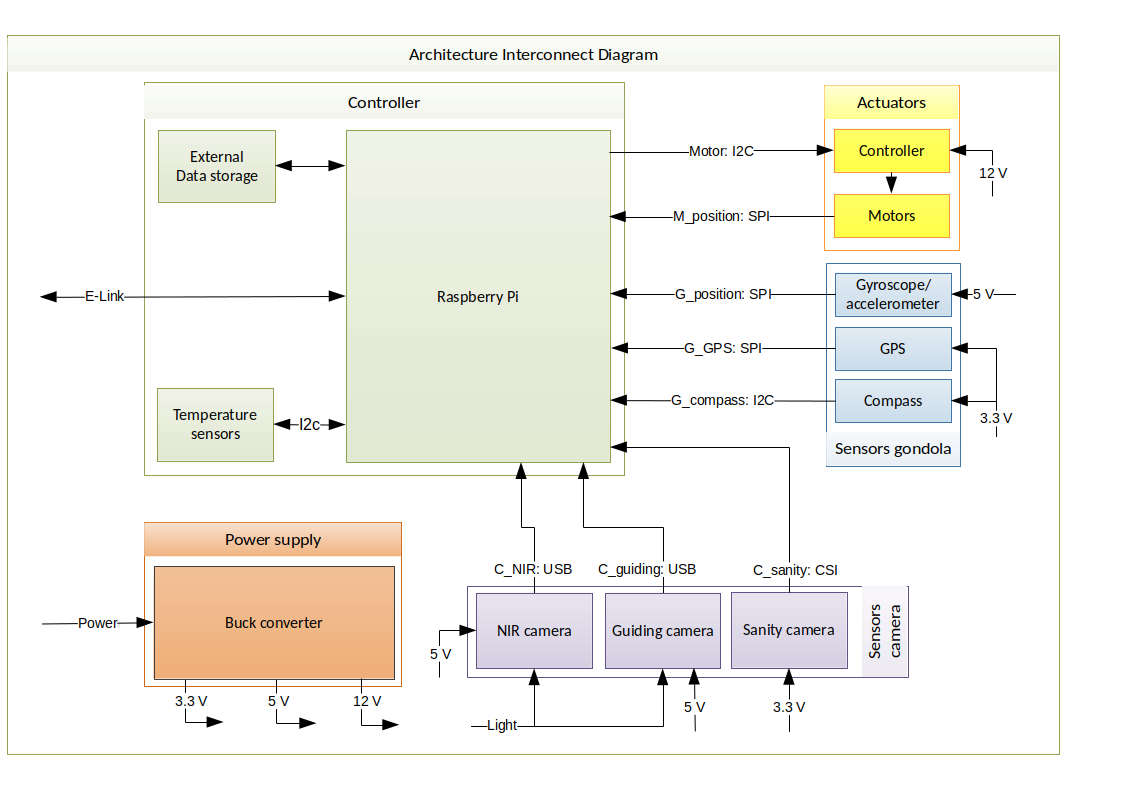
\includegraphics[width=.85\textwidth]{4-experiment-design/img/electrical/ArchitectureInterconnect.png}
	\caption{Electrical architecture interconnect diagram.}
	\label{fig:elec-AID}
\end{figure}

\subsubsection{Motor-controller \& Motor}
\colorbox{yellow}{\parbox{\textwidth}{
When putting a PWM signal on a DC-motor, the position of the DC-motor can be controlled as well as the speed between two positions. The inputs of the motors will always be inverted to each other. This is how a servo motor works as well and will be implemented to position the telescope.\\

The amount of steps per duty cycle of the pwm signal is 12 bits with the PCA9685 chip. This means $2^{12}$ steps between full on and full off. This will result that the motors can turn very very slowly.\\

Then the signal will be amplified in current with a L298 motor driver (H-bridge). This signal will be delivered to a DC-motor which is geared with 1:312. There will be an encoder before and after the gearbox. As most high encoders aren't able to measure below 5 arcseconds. Measuring before the gearbox helps to take smaller steps.\\

The chosen encoder is an AMT23. This encoder has $2^{14}$ positions. When measuring before the gearbox, each step corresponds with 0.25 arcseconds. But because the motor can bounce between two bits the effective resolution is 0.5 arcseconds. The second encoder behind the gearbox has at least 312 steps per rotation, this way the position of the telescope can be measured exactly. Since the encoders are absolute encoders and measure independently of the OBC, a watchdog reboot will not affect these measurements.
}}

\subsubsection{Gyroscopes}
\colorbox{yellow}{\parbox{\textwidth}{
We are currently talking to Honeywell to borrow the GG1320AN Digital Ring Laser Gyroscopes. This will improve the design by a lot and the previous designed gyroscopes below will no longer be used.\\

The current defined gyroscope is the ADXRS624. The main parameter is the noise from the gyroscope is the noise, which is 0.04\,$^\circ/ \sqrt{f_s}$, with $f_s$ being the sampling frequency. This means that a sampling frequency of 80 kHz, this system should be able to stay within the 0.5 arcseconds accuracy. For redundancy it might be necessary to have a dedicated microcontroller for the signal processing. This chip can only measure differences from its 0$^\circ$ position up to 75$^\circ$, but this should be sufficient enough as we can reset the 0$^\circ$ position between images.\\

This chip is analog and must be read out by an ADC that is able to read out the signal with a high enough accuracy on that specific sampling frequency. For this the AD7175 ADC is chosen. With a sampling frequency of 250,000\,Hz the effective resolution is 20.1 bits or 8.7\,$\mu$V. The gyroscope gives a change is voltage of 18\,$\mu$V per arcsecond. Thus everything below 9\,$\mu$V should be sufficient to measure with 0.5 arcseconds accuracy.
}}

%\subsubsection{Star tracker}
%TODO : ADD THIS DECRIPTION
%\colorbox{yellow}{\parbox{\textwidth}{}}

\subsubsection{Schematic}
See Appendix c.

\subsubsection{PCB Layout}
There will be three PCB:s, which are listed below:

\begin{itemize}
	\item 	Power system, motor control \& temperature actuator control.
	\item	Accelerometer, GPS, compass, temperature sensors
	\item 	Gyroscopes
\end{itemize}



The two PCB's for the power system, motor control, temperature, accelerometer, GPS and compass, will be located in the electronics box. They will be placed on top of each other. Also the controller will be mounted in this electronics box. %, see figure \ref{fig:electronic-box}

%\begin{figure}[H]
%	\centering
%	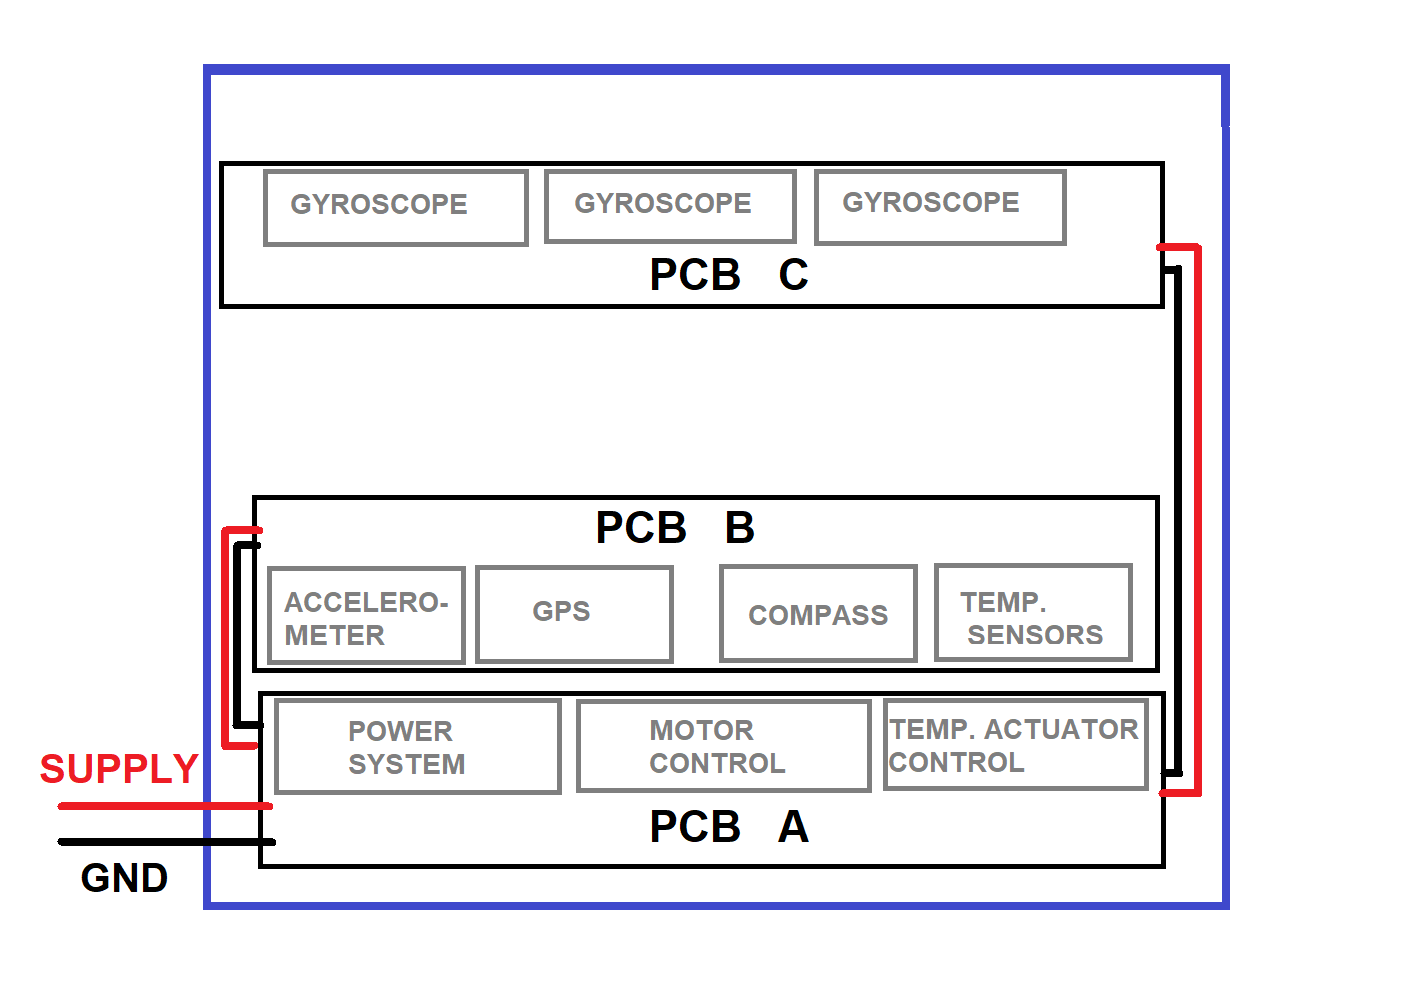
\includegraphics[width=\textwidth]{4-experiment-design/img/electrical/ElectricalBox.png}
%	\caption{An architecture diagram of the electronics.}
%	\label{fig:electronic-box}
%\end{figure}


The third PCB will be placed in its own second electronics box because it includes the gyroscopes. Thus the PCB should not be too close to the other PCBs or the DC motors due to disturbances, such as for example magnetic field changes. The schematics of all the PCBs can be found in appendix C.
\raggedbottom
